%%%%%%%%%%%%%%%%%%%%%%%%%%
%%% author : Yamada. T %%%
%%% made for TH series %%%
%%%%%%%%%%%%%%%%%%%%%%%%%%

\documentclass[b5paper,10pt,fleqn] {ltjsarticle}

\usepackage[margin=10truemm]{geometry}

\usepackage{pict2e, graphicx}
\usepackage{tikz}
\usetikzlibrary{intersections,calc,arrows.meta}

\usepackage{amsmath, amssymb, amsthm}
\usepackage{ascmac}
\usepackage{comment}
\usepackage{empheq}
\usepackage[shortlabels,inline]{enumitem}
\usepackage{fancybox}
\usepackage{fancyhdr}
\usepackage{here}
\usepackage{lastpage}
\usepackage{listings, jvlisting}
\usepackage{fixdif}

\usepackage{stmaryrd}
\usepackage[listings]{tcolorbox}
%\usepackage{ascolorbox}
\usepackage{titlesec}
\usepackage{ulem}
\usepackage{url}
\usepackage{verbatim}
\usepackage{wrapfig}
\usepackage{xcolor}
\usepackage{luatexja-ruby}
\usepackage{varwidth}
\usepackage[version=3]{mhchem}
\usepackage{wrapfig}


\usepackage{physics2}
	\usephysicsmodule{ab}
	\usephysicsmodule{ab.braket}
	\usephysicsmodule{ab.legacy}
	%\usephysicsmodule{braket}
	\usephysicsmodule{diagmat}
	\usephysicsmodule{xmat}
	\usephysicsmodule{nabla.legacy}
	\usephysicsmodule{qtext.legacy}

\usepackage[ISO]{diffcoeff}
\difdef { f, s } { D }
{ op-symbol = \mathrm{D} }


\newcommand{\mctext}[1]{\mbox{\textcircled{\scriptsize{#1}}}}
\newcommand{\ctext}[1]{\textcircled{\scriptsize{#1}}}
\newcommand{\ds}{\displaystyle}
\newcommand{\comb}[2]{{}_{#1}\mathrm{C}_{#2}}
\newcommand{\hs}{\hspace}
\newcommand{\vs}{\vspace}
\newcommand{\emphvs}{\vspace{1em}\notag\\}
\newcommand{\ora}{\overrightarrow}
\newcommand{\ol}{\overline}
\newcommand{\oramr}[1]{\overrightarrow{\mathrm{#1}}}
\newcommand{\tri}{\triangle}
\newcommand{\mr}{\mathrm}
\newcommand{\mb}{\mathbb}
\newcommand{\mrvec}[1]{\overrightarrow{\mathrm{#1}}}
\newcommand{\itvec}{\overrightarrow}
\newcommand{\bs}{\boldsymbol}
\newcommand{\ra}{\rightarrow}
\newcommand{\Ra}{\Rightarrow}
\newcommand{\lra}{\longrightarrow}
\newcommand{\Lra}{\Longrightarrow}
\newcommand{\la}{\leftarrow}
\newcommand{\La}{\Leftarrow}
\newcommand{\lla}{\longleftarrow}
\newcommand{\Lla}{\Longleftarrow}
\newcommand{\lr}{\leftrightarrow}
\newcommand{\llr}{\longleftrightarrow}
\newcommand{\Llr}{\Longleftrightarrow}
\renewcommand{\deg}{{}^\circ}
\newcommand{\phbox}{\fbox{\phantom{1\hspace{2em}}}}
\newcommand{\boxnum}[1]{\fbox{\phantom{\hspace{1em}}({#1})\phantom{\hspace{1em}}}}
\newcommand{\boxkana}[1]{\fbox{\phantom{\hspace{1em}}{#1}\phantom{\hspace{1em}}}}
\newcommand{\boxkm}[2]{\fbox{\, {#1}\phantom{\hspace{0.2em}} \,  {#2}}}
\newcommand{\hzw}{\hspace{1\zw}}

\renewcommand{\baselinestretch}{1.25}
\parindent=1\zw

%入70
\begin{document}
\noindent
\fbox{NewTH1-13} [九州大2008]

\begin{wrapfigure}{r}{5cm}
  \centering
  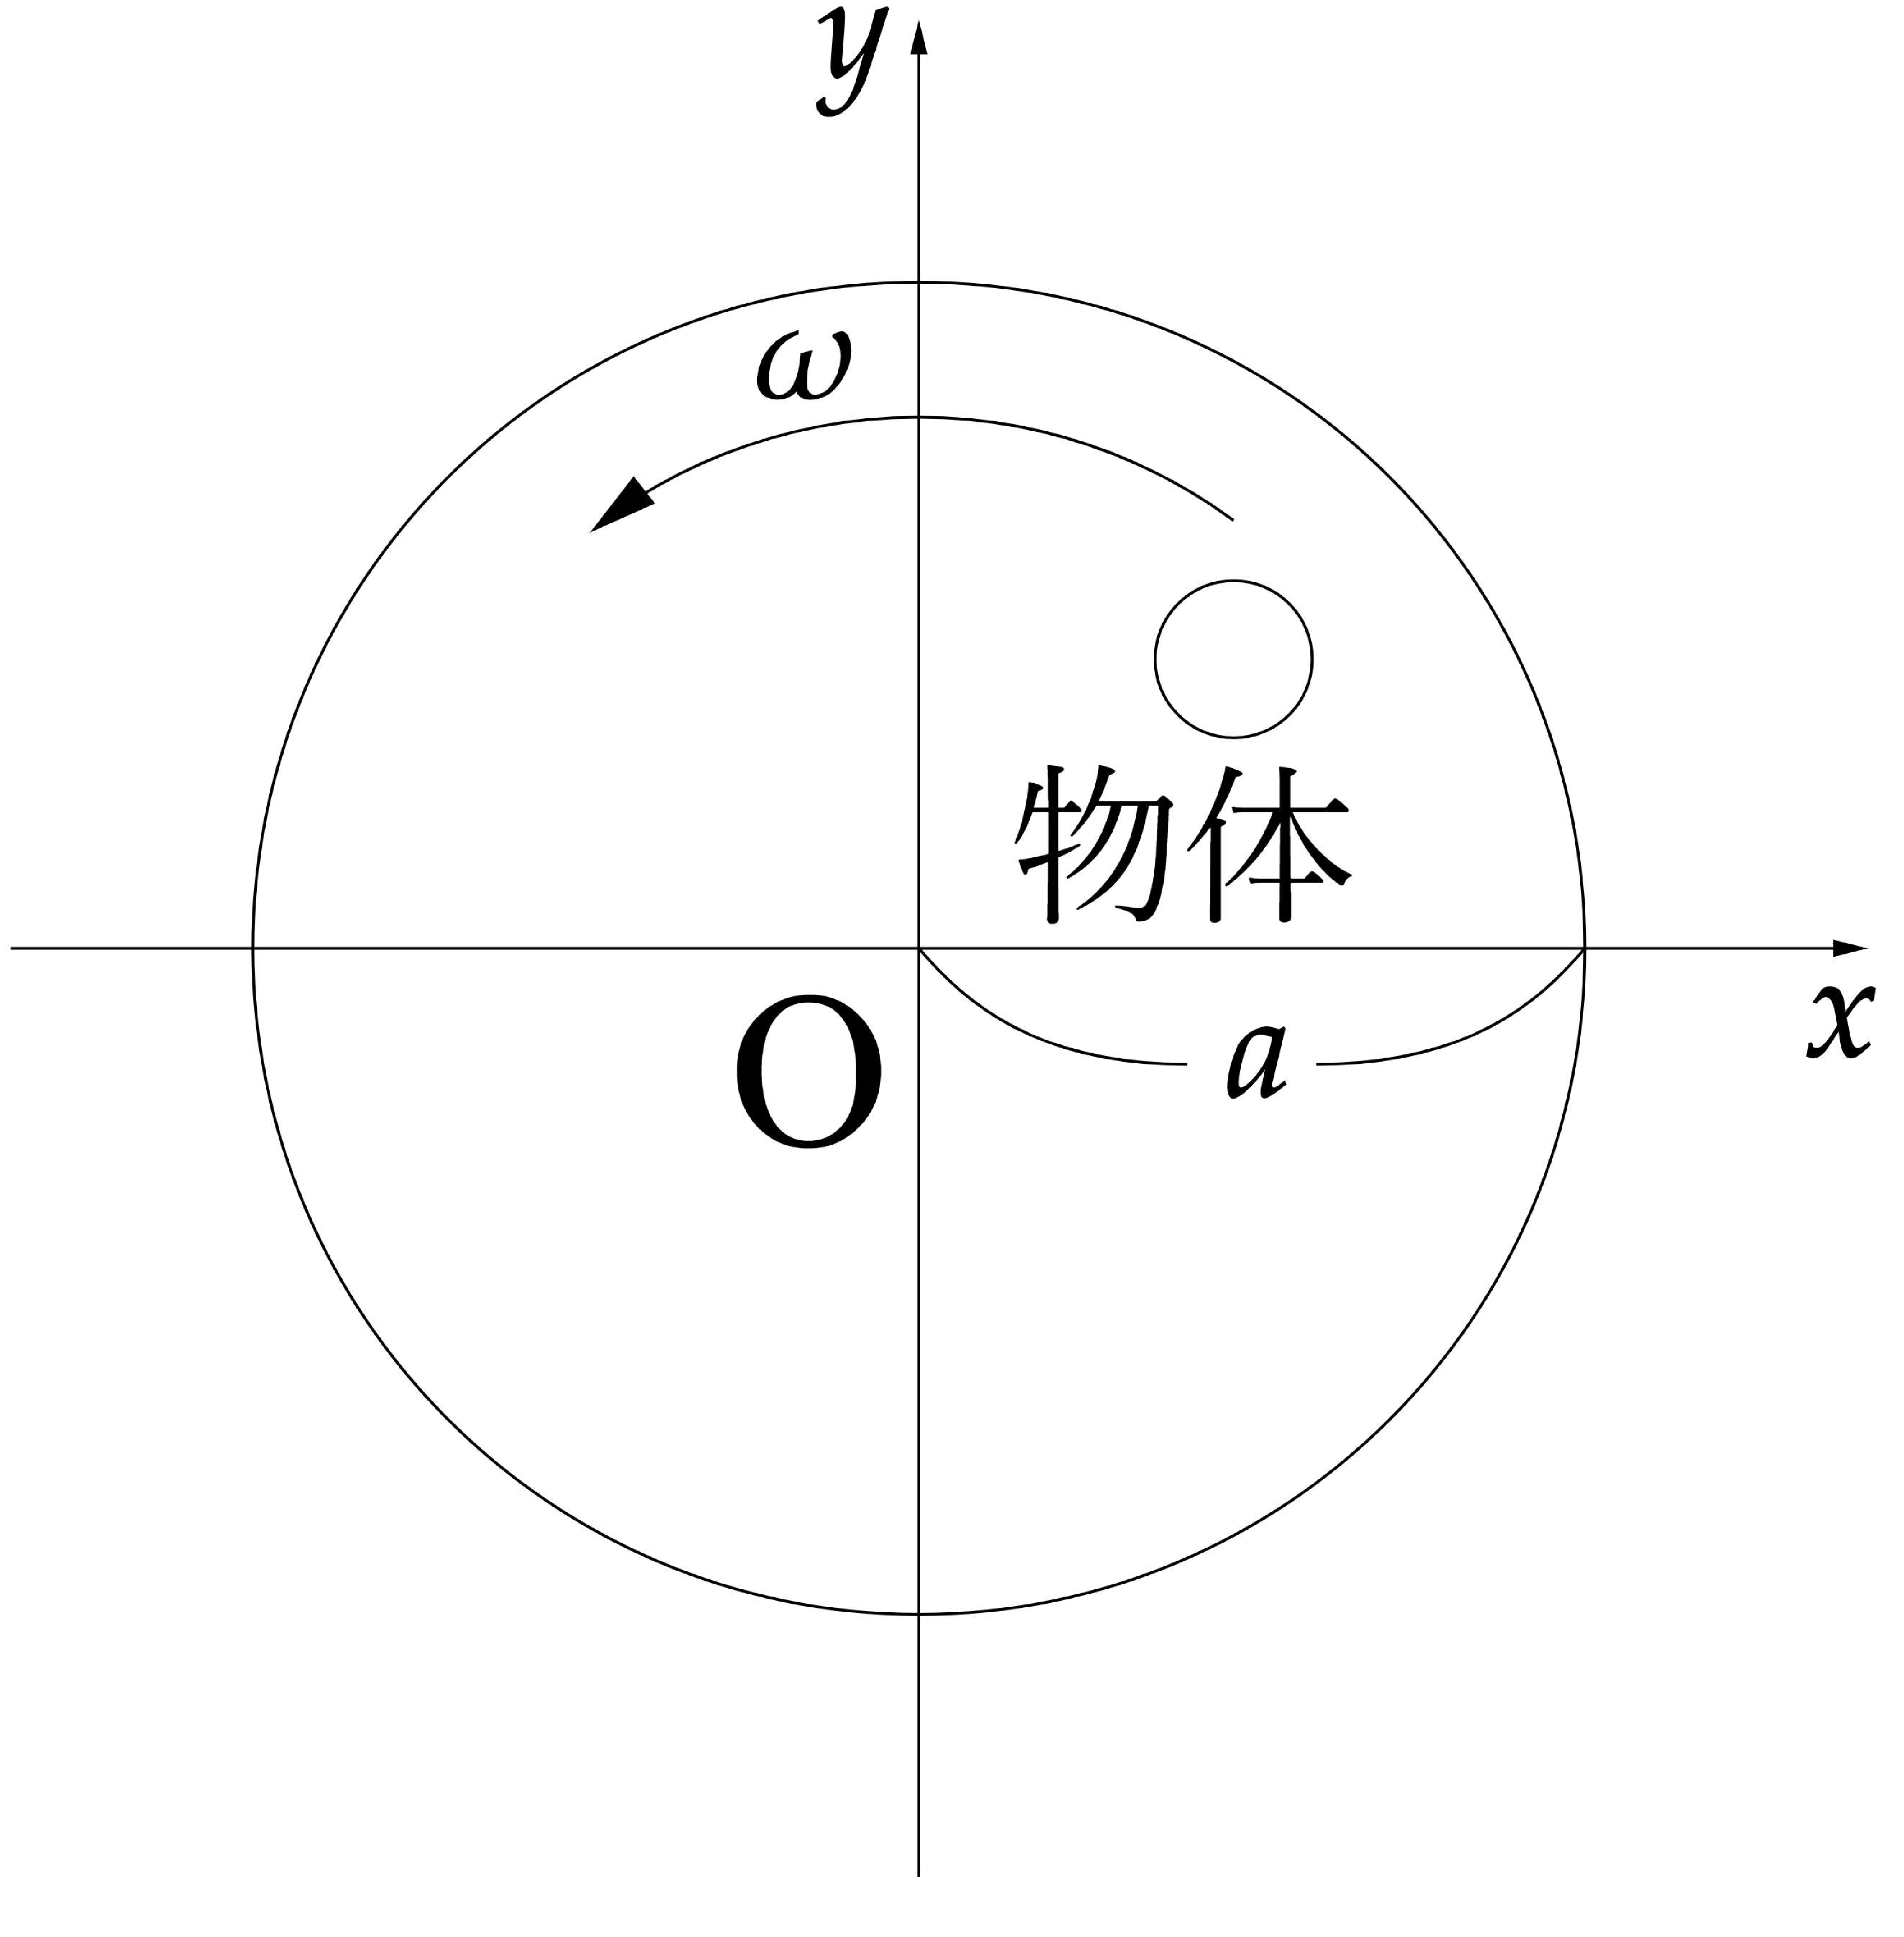
\includegraphics[width=5cm]{fig/fig_1_13_1.pdf}
  \caption{}
\end{wrapfigure}
図1に示すように,静止している水平面($xy$平面)の上に厚さが無視できる半径$a$の円板を置く.円板の中心は原点Oと一致している.円板上に大きさが無視できる質量$m$または$2m$の物体を置き,円板を点Oを中心として反時計回りに回転させる.回転の角速度$\omega$を徐々に大きくしていくと,角速度が小さいとき物体は円盤とともに回転するが,ある角速度で物体は円板に対して動き始める.


円板の角速度変化はゆっくりであり,円板とともに回転する物体の運動は常に等速円運動とみなせるとする.物体と回転円板および静止水平面との間の静止摩擦係数を$\mu$,動摩擦係数を$\mu'$とする.重力加速度の大きさを$g$とし,空気抵抗は無視する.また.角度および角速度の単位は,それぞれ$\mr{rad}$および$\mr{rad/s}$とする.

\begin{enumerate}[label=\textbf{問\arabic*}]
  \item {\hzw}以下の問いに答えよ.
  \begin{enumerate}[(1)]
    \item {\hzw}質量$m$の物体を円板の円周上に置いたとき,物体が円板に対して動き始める直前の角速度$\omega_\mr{A}$を$a$,$g$,$m$,$\mu$,$\mu'$のうち必要なものを用いて求めよ.
    \item {\hzw}質量$2m$の物体を円板の円周上に置けば,物体が円板に対して動き始める角度$\omega_1$は$\omega_\mr{A}$の何倍になるか.
    \item {\hzw}質量$m$の物体を,点Oからの距離が$\dfrac{a}{2}$となるように円板上に置いたとき,物体が円板に対して動き始める角速度$\omega_2$は$\omega_\mr{A}$の何倍になるか.
  \end{enumerate}
  \begin{minipage}{0.6\linewidth}
  \item
      {\hzw}次に,図2に示すように,点Oからの距離が$\sqrt{2}a$で$y$軸に垂直である壁を置き,問1の(1)と同じく,円板の円周上に質量$m$の物体を置いて円板を回転させた.円板の角速度が$\omega_\mr{A}$に達したとき物体は円盤から離れ,静止水平面上を運動して壁面上の点P$(0, \sqrt{2}a)$で壁と衝突した.以下の(2),(3),(4)では$\omega_\mr{A}$および$a$,$g$,$m$,$\mu'$のうち必要なものを用いて解答せよ.
    \end{minipage}
    \begin{minipage}{0.3\linewidth}
    \setlength\abovecaptionskip{-3em}
    \begin{figure}[H]
      \centering
      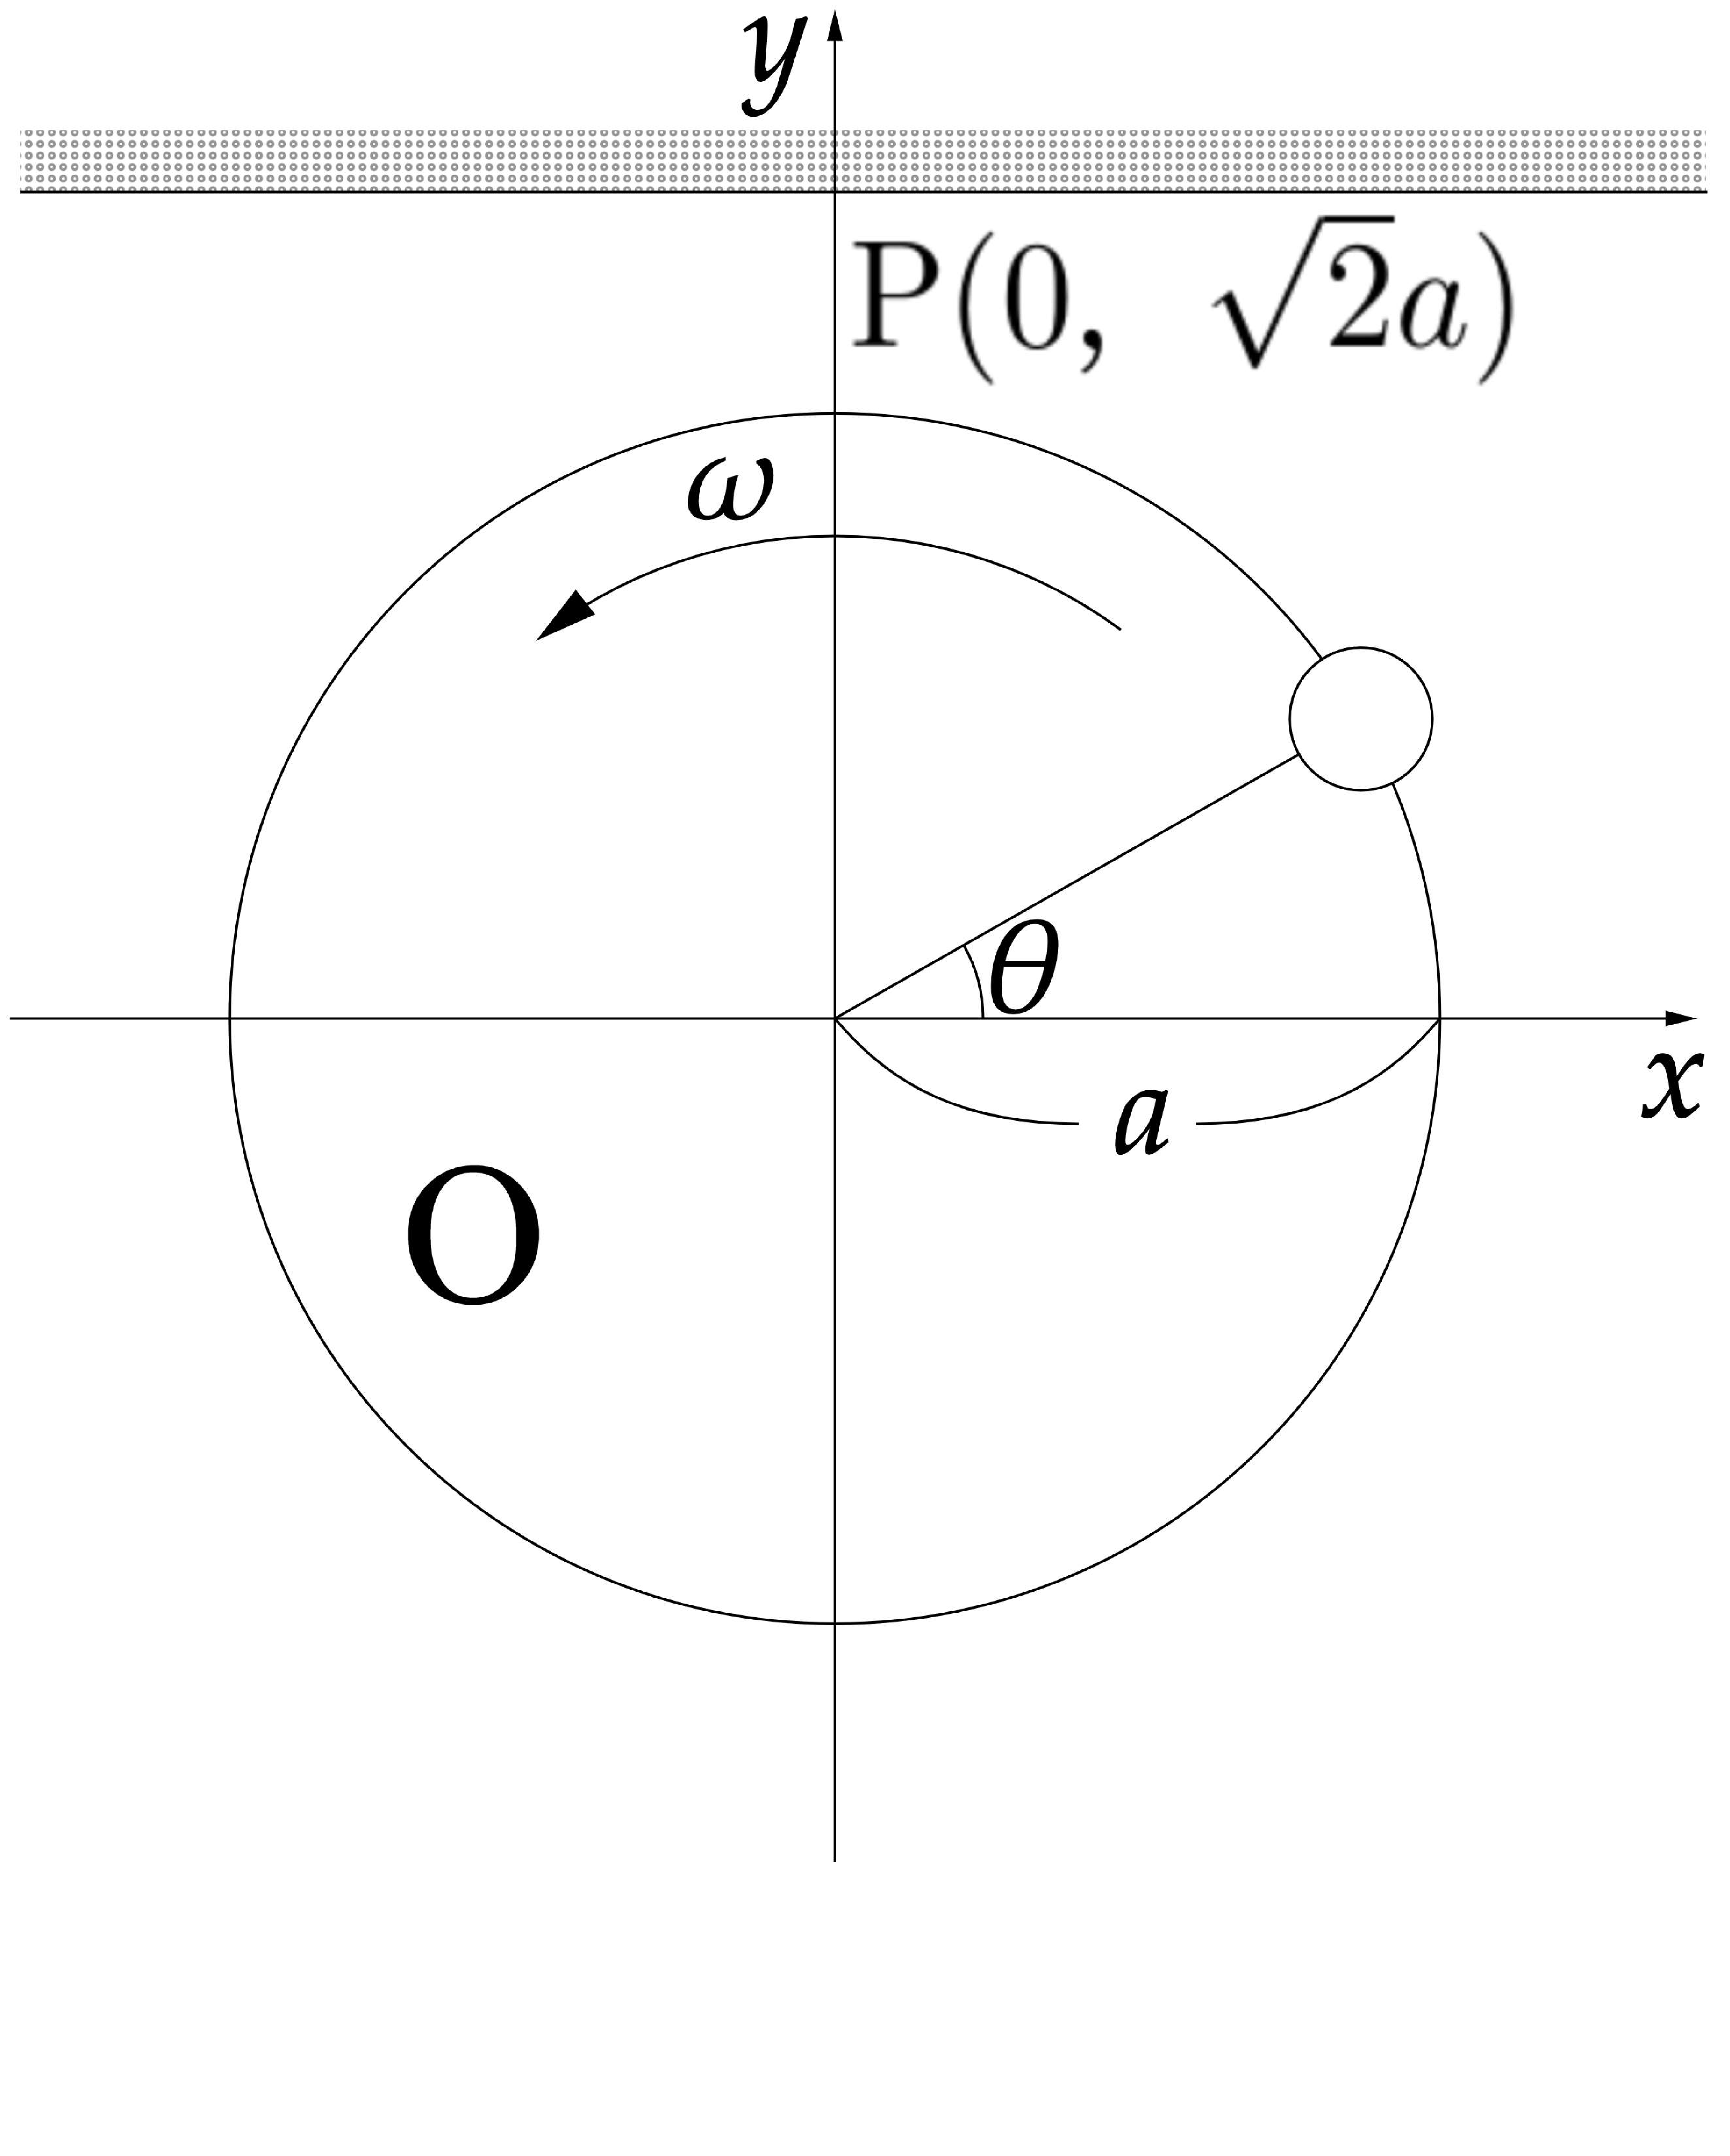
\includegraphics[width=4.5cm]{fig/fig_1_13_2.pdf}
      \caption{}
    \end{figure}
    \end{minipage}
  \begin{enumerate}[(1)]
    \item {\hzw}物体が円盤から離れる瞬間に,物体と点Oを結ぶ線分が$x$軸となす角の大きさ$\theta$はいくらか.
    \item {\hzw}物体が点Pに到達するために必要な$\omega_\mr{A}$に関する条件を求めよ.
    \item {\hzw}物体が円板から離れた後,点Pで壁と衝突するまでの時間$t$を求めよ.
    \item {\hzw}点Pで衝突する直前の物体の速さ$v_1$を求めよ.
  \end{enumerate}
  \item {\hzw}物体は壁面上の点Pで非弾性衝突をした後,静止水平面上を距離$l$だけ運動して静止した.壁の表面はなめらかであり,物体と壁とのはねかえり係数(反発係数)を$e$とする.以下の問いでは,衝突直前の物体の速さ$v_1$および$e$,$g$,$\mu'$のうち必要なものを用いて解答せよ.
  \begin{enumerate}[(1)]
    \item {\hzw}物体が壁に衝突した直後の速度ベクトルを$v_2$とするとき,その$x$方向成分$v_{2x}$および$y$方向成分$v_{2y}$をそれぞれ求めよ.
    \item {\hzw}物体が点Pで衝突した後,静止するまでに運動した距離$l$を求めよ.
  \end{enumerate}
\end{enumerate}
\end{document}
